% Dans l'introduction, on présente le problème étudié et les buts
% poursuivis. L'introduction permet de faire connaître le cadre de la
% recherche et d'en préciser le domaine d'application. Elle fournit
% les précisions nécessaires en ce qui concerne le contexte de
% réalisation de la recherche, l'approche envisagée, l'évolution de
% la réalisation. En fait, l'introduction présente au lecteur ce
% qu'il doit savoir pour comprendre la recherche et en connaître la
% portée.

\Chapter{INTRODUCTION}\label{sec:Introduction} 
The growing accessibility to robots has enabled the rise of the new field of swarm robotics. It corresponds to the application of swarm intelligence to the field of robotics and will be detailed below in section \ref{sec:Introduction:basic}. Robot swarms are particularly appealing for exploration missions involving large and unknown environments where a team effort can yield better results. Indeed, with proper coordination between the robots, the exploration rate should increase proportionally with the number of team members~\cite{burgard2005coordinated}. We define by exploration the action of covering an unknown environment and gathering information about it. Swarm systems should in theory be less prone to failures because of their inherent redundancy. However, it has been demonstrated that in practice, they do not benefit of this property and are, in some cases, even less reliable than traditional centralized robots systems in the presence of risk~\cite{bjerknes2013fault}. Designing specific tools for risk management in swarm systems is therefore of high importance~\cite{prorok2021beyond} and has been the primary focus of this master's degree. This thesis 
presents two algorithms that improve tolerance to risk in robot swarm exploration. The first, named \ac{DORA-Explorer}, is a risk-aware exploration algorithm that minimizes the risk to which robots expose themselves while maximizing the amount of terrain covered, which is published as: 

\shadowbox{%
\begin{minipage}[l]{.99\textwidth}
D Vielfaure, S Arseneault, P-Y Lajoie, G Beltrame. ``DORA: Distributed Online Risk-Aware Explorer''. 2022.  IEEE International Conference on Robotics and Automation (ICRA).
\end{minipage}}

The second algorithm, \ac{RASS}, introduces risk-awareness at the storage and routing level of the swarm by levering a fitness policy based both on risk and hop-count, and was published as:

\shadowbox{%
\begin{minipage}[l]{.99\textwidth}
S Arseneault, D Vielfaure, G Beltrame. "RASS: Risk-Aware Swarm Storage". 2022.  International Conference on Autonomous Agents and Multiagent Systems (AAMAS).
\end{minipage}}

These two algorithms can be used on their own or side-by-side and are intended to improve the resilience of robots swarms carrying exploration missions in dangerous environments.


\section{Definitions and Basic Concepts}
\label{sec:Introduction:basic} 
%The basic concepts upon which the algorithms DORA-Explorer and RASS are built are presented in the following section.

Swarm intelligence is a discipline that focuses on the mechanisms leading to global order in systems composed of many individuals coordinating through local interactions. Swarm intelligence can be seen in both natural and artificial systems where the collective behaviors are obtained in a fully decentralized fashion. Many examples of such systems can be found in nature, for example colonies of ants, schools of fish, flocks of birds or herds of land animals~\cite{Dorigo:2007}. Systems that fall into the discipline of swarm intelligence display the following characteristics: 

\begin{itemize}
    \item A swarm system comprises many individuals and should be able to adapt to varying quantities of individuals
    \item There is no central coordination, agents' behaviors emerge only from local interactions
    \item The system is greater than the sum of its individuals. In other words, when taken individually, the agents are relatively incapable but collectively they achieve impressive results
\end{itemize}

Such characteristics result in an adaptable system that should, in theory, display better tolerance to risk. Indeed, the absence of central coordination not only eliminates a bottleneck that could limit scalability, it also removes a central point of failure that could compromise the entire system if taken down.

As for swarm robotics, it falls into the artificial category of swarm intelligence and more specifically corresponds to the application of the discipline to the field of robotics. It is at the intersection of collective robotics and swarm intelligence. Of course, because of the engineering nature of swarm robotics, physical limitations arise. Bandwidth restrictions, communication capabilities, storage limitations and physical constraints all need to be taken into account when designing robot swarm systems. Additionally, swarm robotics needs to respect some design principles to adhere to the characteristics of swarm intelligence. Specifically, there must be no centralized control, no predefined roles and the global behavior needs to emerge from simple and local interactions.

\section{Problem Elements}
Recently, a lot of attention from the research community has been oriented towards risk-aware autonomous systems. Taking risk into account when designing robot systems is of capital importance as they are increasingly deployed on real-world scenarios with safety-critical applications, including the transportation sector, aerospace systems or collaborative manufacturing. These robotic systems evolve in uncontrolled environments and must face risks on a daily basis, motivating the need for risk awareness. Excessive risk taking, or a complete absence of considering it, may not only jeopardize the robotic system, it may also endanger components in its vicinity and possibly human lives. For robot swarms tasked with the exploration of unknown environments, risk is generally location-based and takes the form of environmental hazards. Other types of risk exist, however this work focuses on risk that arises from interactions with the environment and corresponds to interactions faults from section \ref{sec:faultdetection}. The exploration of hazardous environments using teams of robots comes with its own set of advantages and constraints. Carrying the exploration mission with numerous robots should result in faster terrain coverage than in a single robot mission~\cite{burgard2005coordinated}.  However, failures can considerably reduce the performance of the team and should therefore by avoided as much as possible. Not taking risk into account when exploring will inevitably lead to a decrease in performance of the team. 

\subsection{Terrain Coverage}
\label{sec:problemCoverage}

Applied to a scenario of terrain coverage, the problem element of not considering risk is presented in figures \ref{statementDORA1} and \ref{statementDORA2}. In figure \ref{statementDORA1}, robots of the team start exploring the environment by covering as many cells as possible. After a while, in figure \ref{statementDORA2}, robots start experiencing failures due to environmental hazards. In this example, risk takes the form of point radiation sources, however, any other type of danger could be considered (e.g., rough terrain or fire). Because of failures, the number of team members carrying the exploration mission decreases drastically. As a result, the exploration rate decreases and large portions of the environment remain uncovered. The intuition shown in figures \ref{statementDORA1} and \ref{statementDORA2} presents DORA-Explorer's problem statement. DORA-Explorer tries to solve it by introducing a consciousness of risk in the motion control loop of the robots. 

\begin{figure}[htbp]
	\centering
    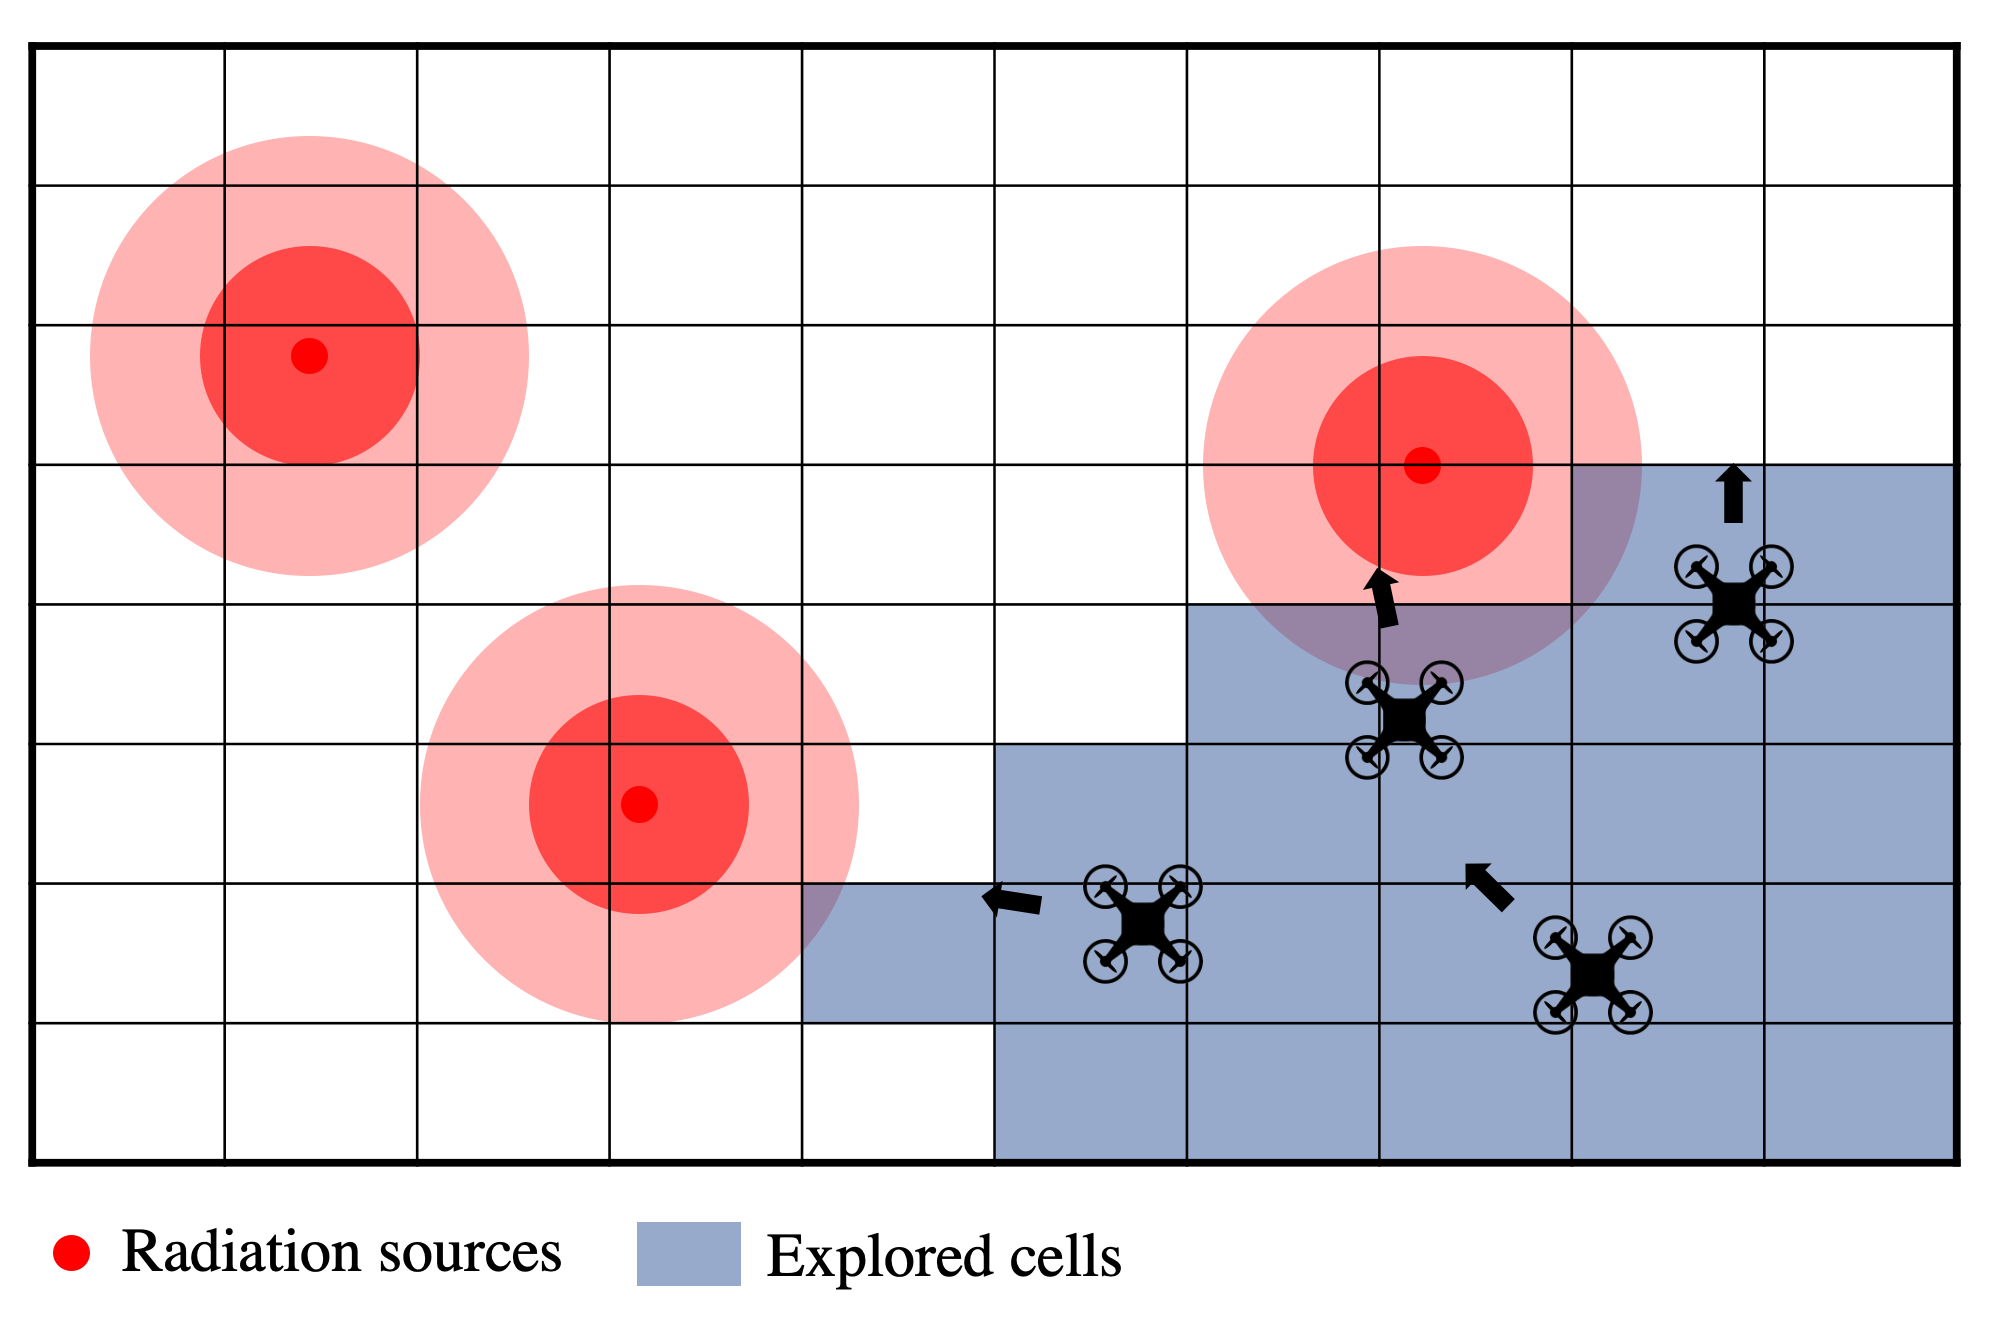
\includegraphics[width=0.70\columnwidth]{images/problemStatement1.png}
    \caption{Exploration of an unknown environment with a team of robots}
    \label{statementDORA1}
\end{figure}

\begin{figure}[htbp]
	\centering
    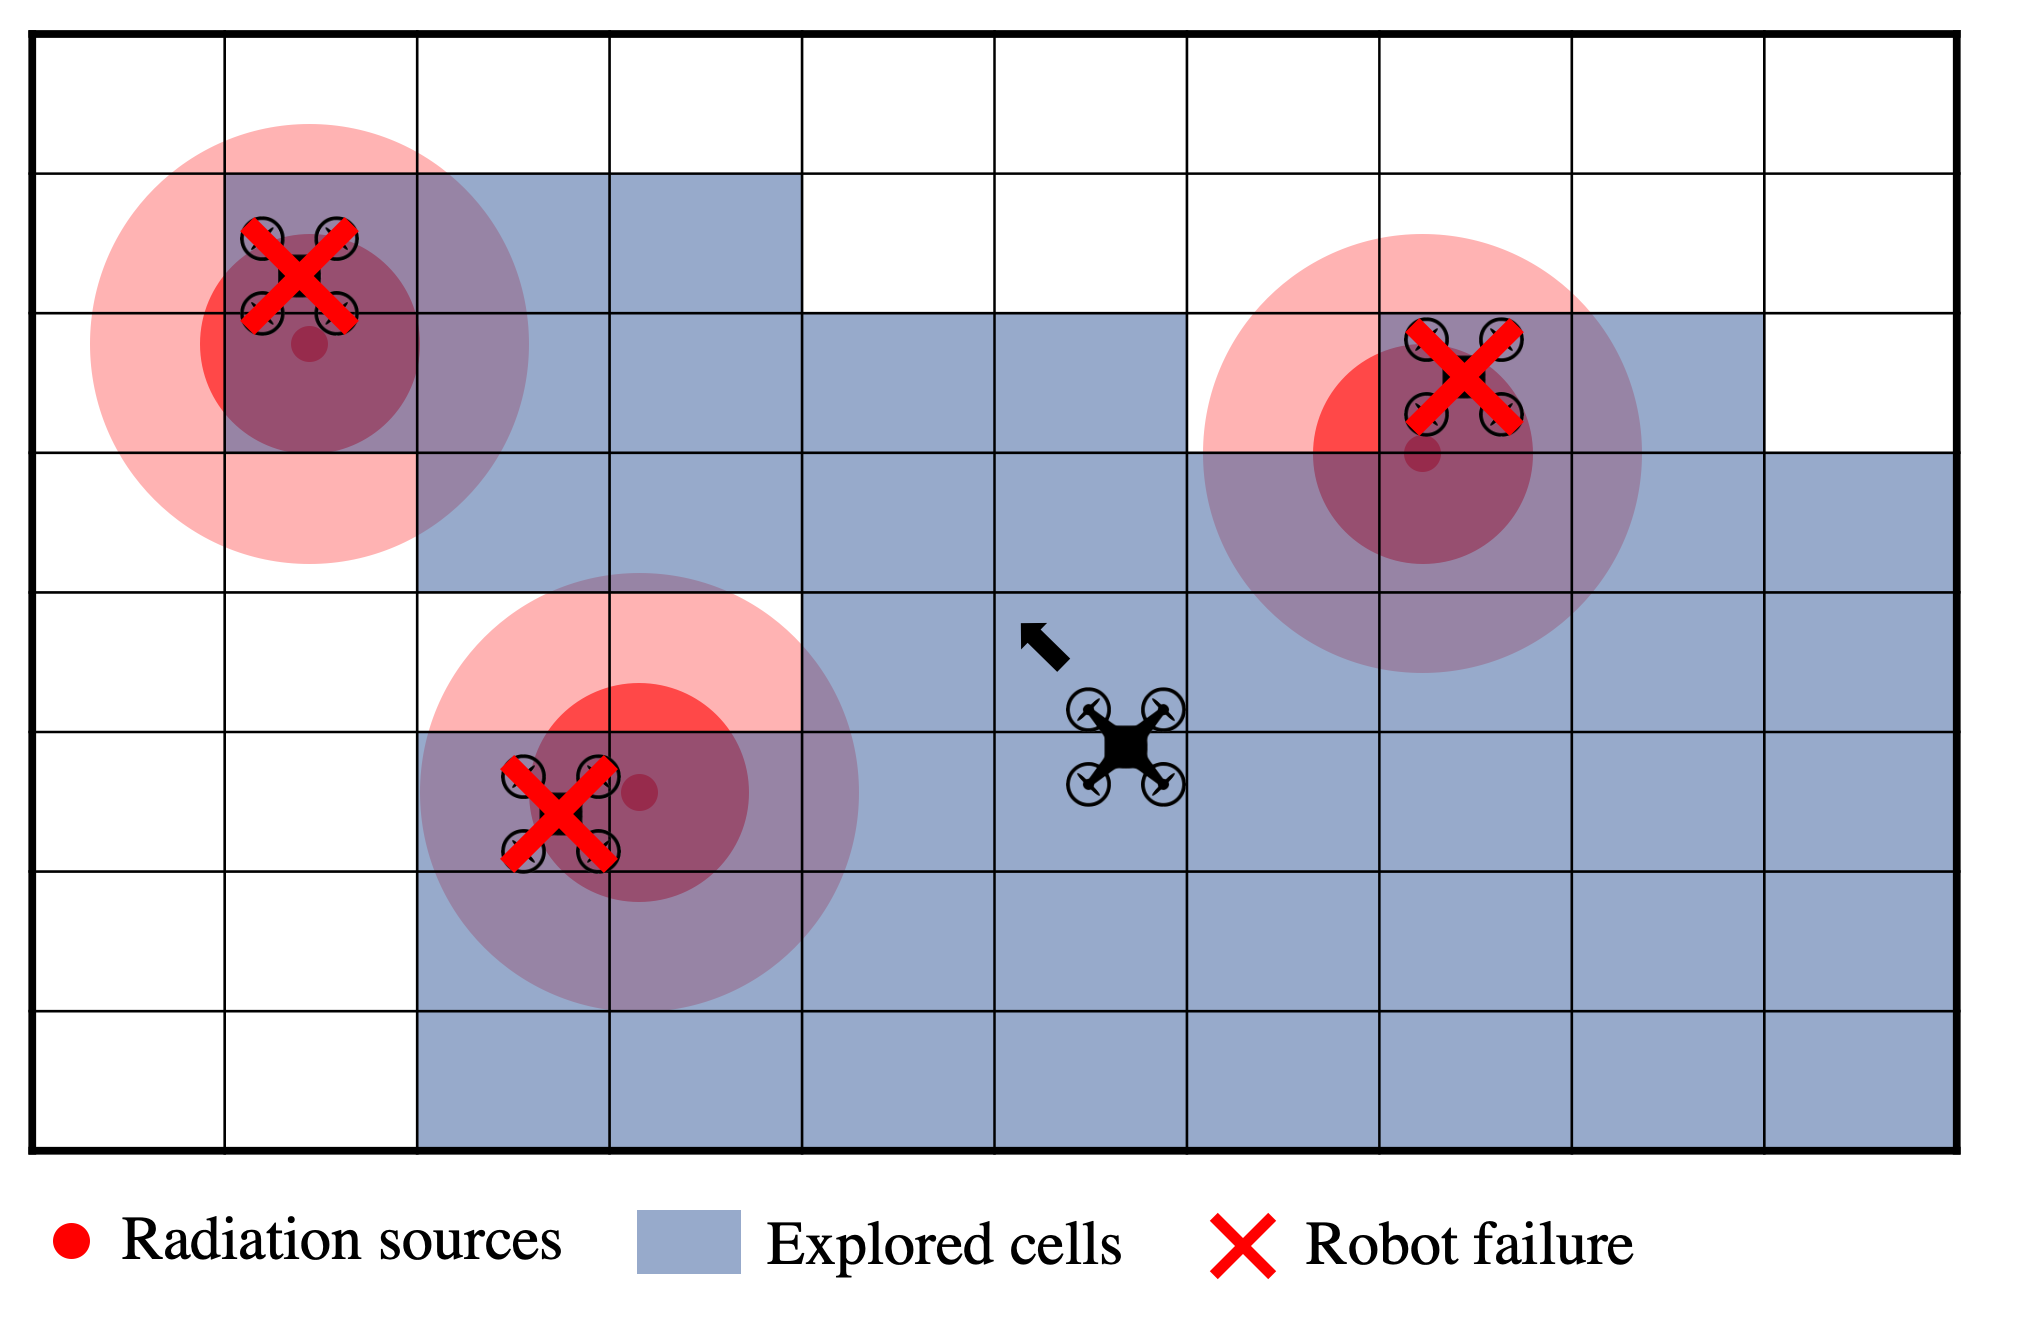
\includegraphics[width=0.70\columnwidth]{images/problemStatement2.png}
    \caption{Exploration of an unknown environment with a team of robots affected by failures.}
    \label{statementDORA2}
\end{figure}


\subsection{Information Gathering}
\label{sec:problemInformation}
Naturally, a similar problem statement can be expressed in terms of information gathering. Again, carrying the mission with numerous robots should result in a faster information gathering. However, if robots collecting information are susceptible to data corruptions, not taking risk into account will lead to inferior data collection performances. This is especially true for robot swarms operating in poorly connected environments, where directly sending the acquired data items to permanent external storage is not always possible. The robots often need to store the information locally and the robotic system acts as a temporary storage infrastructure. Assuming that environmental hazards might compromise some of the robots of the system, determining which ones are the best-suited for storing information becomes essential for reducing the likelihood of data losses. This intuition is presented in Figure \ref{statementRASS}. In figure \ref{statementRASS}, robots are dispatched in an unknown environment with the task of gathering information about it. Because the environment contains dangers, in our case a point radiation source, data items collected by robots may become corrupted if exposed to it. Transiting collected data items through robots located near a radiation source will therefore increase the likelihood of corruption. In figure \ref{statementRASS}, the lower route, although more direct towards the base station, is definitely more dangerous than the upper one. To reduce the likelihood of data losses, robots could use the upper route to reach the base station. This is the problem statement of RASS, the second algorithm of the thesis. RASS solves the problem by avoiding risky nodes of the system in its storage and routing scheme.

\begin{figure}[htbp]
	\centering
    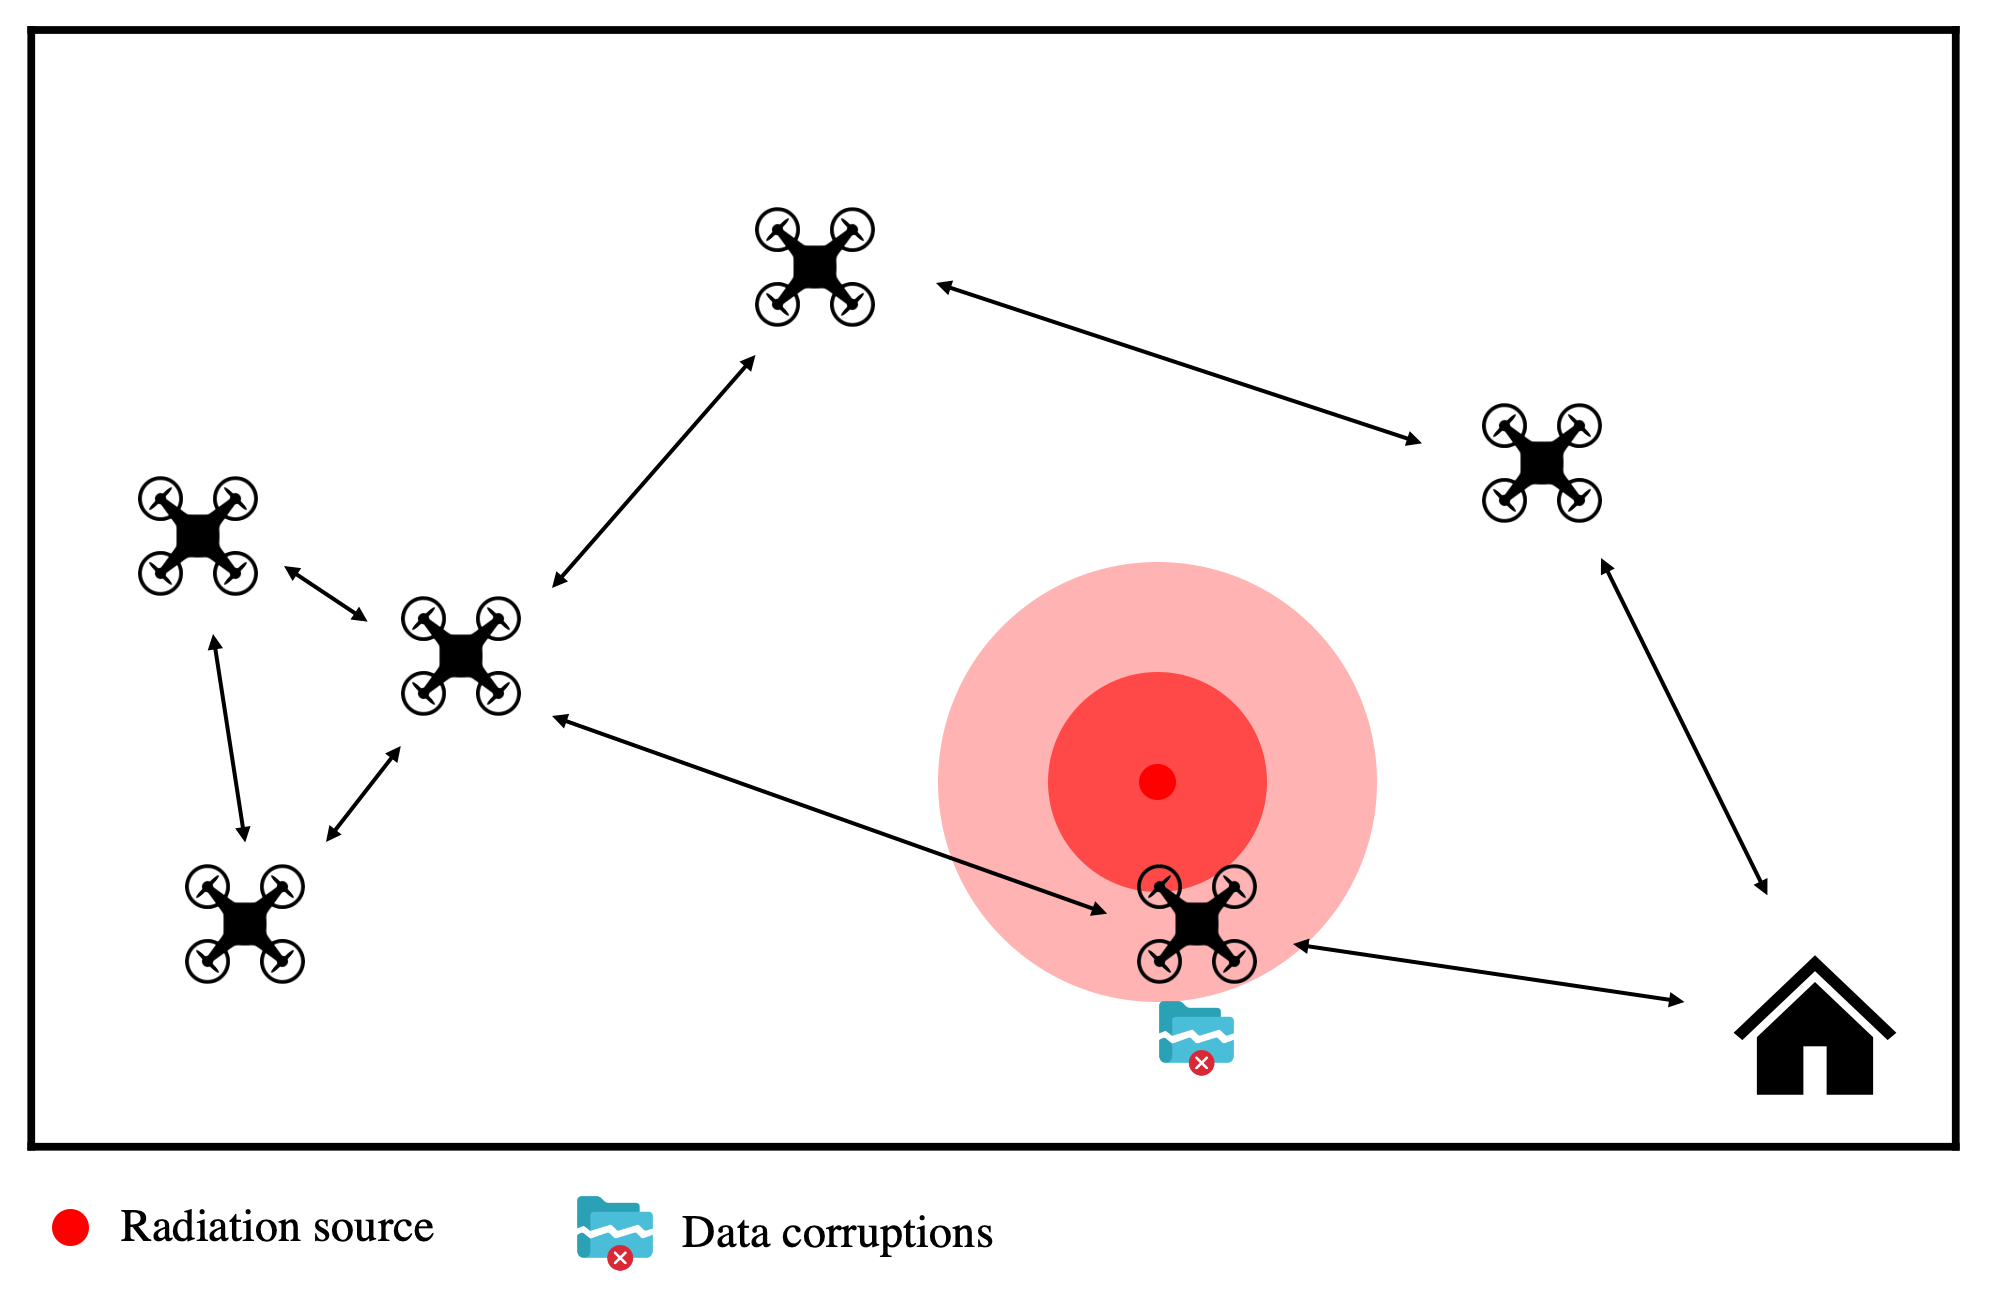
\includegraphics[width=1\columnwidth]{images/statementRASS.png}
    \caption{Information gathering in an hazardous environment}
    \label{statementRASS}
\end{figure}


\section{Research Objectives} 
\label{sec:objectifs}

Developing robot swarm algorithms to perform exploration missions in potentially dangerous environments has been the primary research objective of this master's degree. As mentioned in the previous section, this is of great importance as failures resulting from excessive exposure to risk will inevitably reduce the performance of the swarm. 

\subsection{Risk-aware Coverage}
In this regard, we first focus on bringing risk awareness to a terrain coverage algorithm, something that was lacking in the literature. Explicitly, the developed coverage algorithm should reduce considerably the failure rate of the robots carrying the exploration mission when compared to other state-of-the-art algorithms. Of course, the proposed solution should also achieve comparable terrain coverage performances when compared to these same state-of-the-art algorithms. Because the developed algorithm is intended for robot swarms, it also needs to respect the swarm robotics design principles seen in the previous section. With these objectives in mind, the algorithm should address the problem elements specific to terrain coverage in dangerous environments from section \ref{sec:problemCoverage}. To summarize, the research objectives related to terrain coverage in dangerous environments are listed below:

\begin{compactenum}
    \item Reduce failure rate compared to other state-of-the-art algorithms;
    \item Achieve comparable terrain coverage compared to other state-of-the-art algorithms;
    \item Respect swarm robotics design principles;
    \item Test real-world applicability with experiments on physical robots;
\end{compactenum}


\subsection{Risk-aware Information Gathering}
Second, we focus on risk awareness to the specific problem of information gathering performed in potentially dangerous environments, as seen in section \ref{sec:problemInformation}. The related research objectives are the following: The proposed solution should reduce notably the rate of data items that are lost due to the environmental dangers. Also, the developed solution should provide adequate transfer speeds, defined as the time it takes for data items to reach the base station after creation. Again, it will need to respect the swarm robotics design principles as it is intended to be deploy on robot swarms. To summarize, the research objectives related to information gathering in dangerous environments are listed below:

\begin{enumerate}
    \item Reduce data corruption rate compared to other state-of-the-art algorithms;
    \item Achieve comparable transfer speed compared to other state-of-the-art algorithms;
    \item Respect swarm robotics design principles;
    \item Test real-world applicability with experiments on physical robots;
\end{enumerate}


\section{Thesis outline}
The remainder of the thesis is structured as follows. In chapter \ref{sec:RevLitt}, a literature review of relevant related works is presented. The following topics will be studied in the literature review: swarm robotics, swarm programming, information sharing, routing mechanisms, swarm exploration strategies, risk in swarm robotics and some notable fault detection methods. Following the literature review, in chapter \ref{sec:approach}, the scientific approach used to meet the research objectives will be presented. Then, in chapter \ref{sec:Theme1} the algorithm DORA-Explorer, which uses risk awareness in its exploration strategy, will be presented. Subsequently, chapter \ref{sec:Theme2} will cover RASS, a risk-aware storing and routing mechanism designed for robot swarms carrying exploration missions. A high-level discussion on the results obtained throughout the master's degree in relation with the research objectives will follow in chapter \ref{sec:discussion}. Finally, in chapter \ref{sec:Conclusion}, a conclusion is presented alongside the limitations of the work and interesting future research directions.
